\documentclass[11pt]{article}
\usepackage{graphicx}
\usepackage{enumitem}

%%%%%%%%%%%%%%%%%%%%%%%%%%%%%%%%%%%%%%%%%%%%%%%%%%%%%%%%%%%%%%%%%%%%%%%%%%%%%%%%
% packages
%%%%%%%%%%%%%%%%%%%%%%%%%%%%%%%%%%%%%%%%%%%%%%%%%%%%%%%%%%%%%%%%%%%%%%%%%%%%%%%%

\usepackage{coling2020}
\usepackage{times}
\usepackage{url}
\usepackage{latexsym}
\usepackage{hyperref}
\hypersetup{
  colorlinks   = true, %Colours links instead of ugly boxes
  urlcolor     = blue, %Colour for external hyperlinks
  linkcolor    = blue, %Colour of internal links
  citecolor    = blue  %Colour of citations
}


%%%%%%%%%%%%%%%%%%%%%%%%%%%%%%%%%%%%%%%%%%%%%%%%%%%%%%%%%%%%%%%%%%%%%%%%%%%%%%%%
% paper configuration
%%%%%%%%%%%%%%%%%%%%%%%%%%%%%%%%%%%%%%%%%%%%%%%%%%%%%%%%%%%%%%%%%%%%%%%%%%%%%%%%

%\setlength\titlebox{5cm}
%\colingfinalcopy % Uncomment this line for the final submission

% You can expand the titlebox if you need extra space
% to show all the authors. Please do not make the titlebox
% smaller than 5cm (the original size); we will check this
% in the camera-ready version and ask you to change it back.


\title{Instructions for COLING-2020 Proceedings}

\author{First Author \\
  Affiliation / Address line 1 \\
  Affiliation / Address line 2 \\
  Affiliation / Address line 3 \\
  {\tt email@domain} \\\And
  Second Author \\
  Affiliation / Address line 1 \\
  Affiliation / Address line 2 \\
  Affiliation / Address line 3 \\
  {\tt email@domain} \\}

\date{}

%%%%%%%%%%%%%%%%%%%%%%%%%%%%%%%%%%%%%%%%%%%%%%%%%%%%%%%%%%%%%%%%%%%%%%%%%%%%%%%%
% latex functions
%%%%%%%%%%%%%%%%%%%%%%%%%%%%%%%%%%%%%%%%%%%%%%%%%%%%%%%%%%%%%%%%%%%%%%%%%%%%%%%%


%%%%%%%%%%%%%%%%%%%%%%%%%%%%%%%%%%%%%%%%%%%%%%%%%%%%%%%%%%%%%%%%%%%%%%%%%%%%%%%%
% document text
%%%%%%%%%%%%%%%%%%%%%%%%%%%%%%%%%%%%%%%%%%%%%%%%%%%%%%%%%%%%%%%%%%%%%%%%%%%%%%%%

\begin{document}
\maketitle
\begin{abstract}
\end{abstract}

%
% The following footnote without marker is needed for the camera-ready
% version of the paper.
% Comment out the instructions (first text) and uncomment the 8 lines
% under "final paper" for your variant of English.
% 
\blfootnote{
    %
    % for review submission
    %
    \hspace{-0.65cm}  % space normally used by the marker
    Place licence statement here for the camera-ready version. 
    %
    % % final paper: en-uk version 
    %
    % \hspace{-0.65cm}  % space normally used by the marker
    % This work is licensed under a Creative Commons 
    % Attribution 4.0 International Licence.
    % Licence details:
    % \url{http://creativecommons.org/licenses/by/4.0/}.
    % 
    % % final paper: en-us version 
    %
    % \hspace{-0.65cm}  % space normally used by the marker
    % This work is licensed under a Creative Commons 
    % Attribution 4.0 International License.
    % License details:
    % \url{http://creativecommons.org/licenses/by/4.0/}.
}

\section{Introduction}
\label{sec:intro}
\begin{center}
\begin{figure}[!ht]
  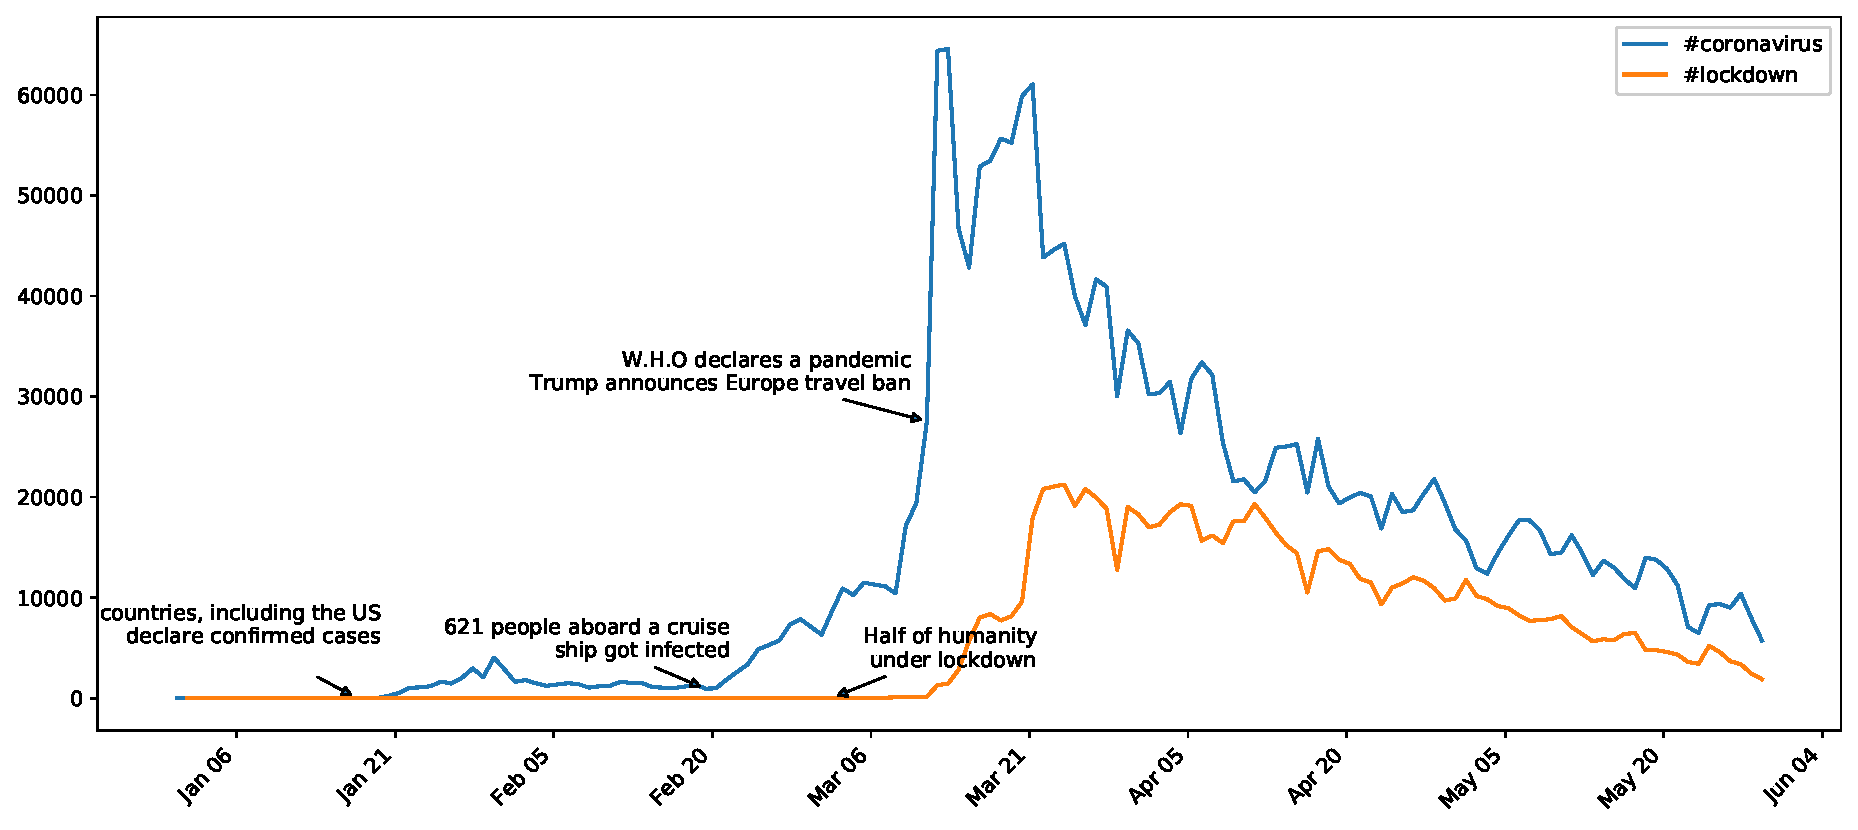
\includegraphics[width=\textwidth]{images/finalcountgraph1.eps}
  \caption{Number of tweets per day...}
  \label{fig:1}
\end{figure}
\end{center}
\newpage

\section{Method Overview}
\label{sec:method}

\section{Experiments}
\label{sec:experiments}


\subsection{Plutchik's Wheel of Emotions}

\begin{figure}[!ht]
    \includegraphics[width=0.4\textwidth]{images/Plutchik-wheel.png}
    \caption{Plutchik's emotion wheel}
    \label{fig:2}
    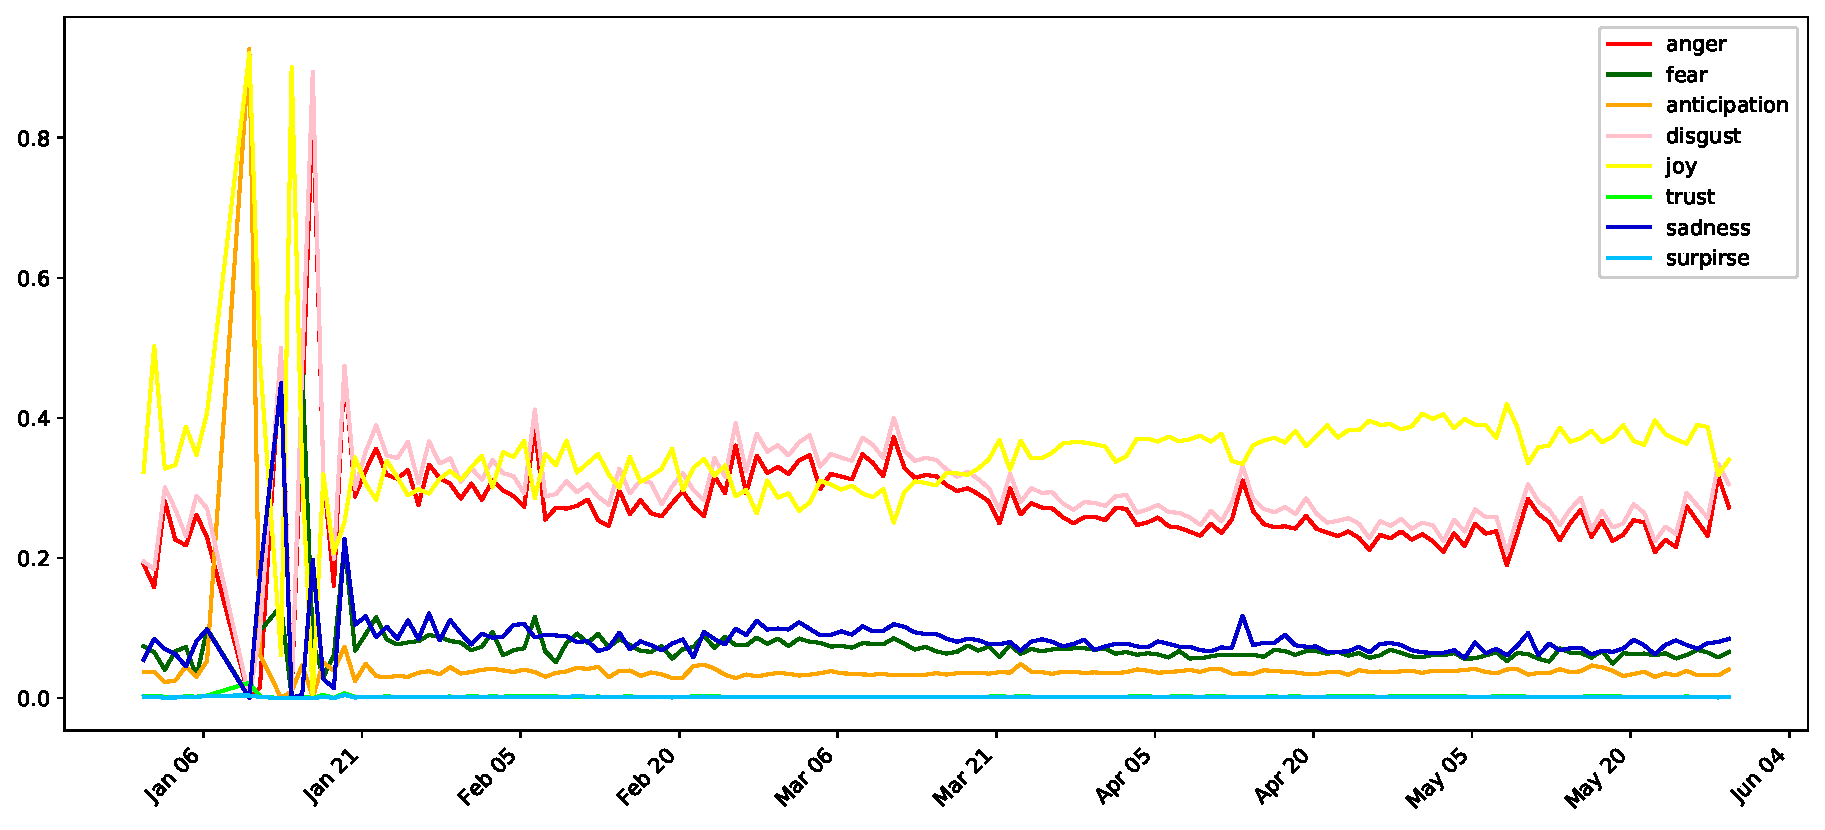
\includegraphics[width=\textwidth]{images/emotions.eps}
    \caption{Results of sentiment analysis conducted using nvidia-sentiment on 170k tweets related with the corona outrbreak }
    \label{fig:3}
\end{figure}
\newpage

\section{Related Work}
\label{sec:related}
\subsection{Stefanos}
Datasets: 

DENS: A Dataset for Multi-class Emotion Analysis:By finetuning the pre-trained uncased BERT-large to a multi-class passage classification task they achieved a micro-F1 score of 60.4\%. 



%\cite{liu2019dens}

%\cite{SemEval2018Task1}

Pretrained models:

%\cite{puri2018large}

%\cite{kant2018practical}

Examples of large scale sentiment analysis:

%\cite{mohammad2015sentiment}

%\cite{hemmatian2017survey}

%\cite{yang2015twitter}


\section{Discussion}
\label{sec:discussion}


\bibliographystyle{coling}
\bibliography{main}

\end{document}
